\chapter{Semantic Search and the RAG Conversational Assistant}
\label{chap:rag}

\section{Overview}
\label{sec:rag-overview}

The preceding chapters describe a serving path that is, by explicit architectural principle, deterministic and free of generative-model calls: the personalized feed (Chapter~\ref{ch:recommendation}) is produced by a fixed weighted formula, not by a language model reasoning about each candidate item. This chapter concerns the one part of AI Compass where that principle is deliberately relaxed: the conversational assistant, which exists because a ranked list of items, however well personalized, cannot answer a free-form question such as ``what does this mean?'' or ``which of these releases support long-context inference?''. The assistant is built on the retrieval-augmented generation (RAG) pattern: a \emph{retrieval} model, running over embeddings of the ingested corpus, selects a small set of passages relevant to the user's question, and a separate \emph{generation} model produces an answer conditioned only on those passages \cite{lewis2020rag}. Retrieval is embedding-based, deterministic given its inputs, and never calls a large language model; generation is the one step in the entire request-serving path that does. Conflating the two would misrepresent AI Compass as an application whose every request passes through a language model, when the ranking and browsing hot path (Chapter~\ref{ch:recommendation}) deliberately does not. The rest of this chapter follows the pipeline in order: chunking and indexing, retrieval and access control, generation and grounding checks, multi-turn conversation, and streaming.

Figure~\ref{fig:screenshot-search} shows the platform's search surface, which is the semantic/keyword search feature referenced above rather than the conversational assistant itself: a query for ``llm quantization techniques'' returning real, currently-indexed arXiv and Reddit results on quantization methods, each carrying its source, category, and topic tags. The assistant itself is a separate, chat-style panel, shown open alongside an article in Figure~\ref{fig:screenshot-rag-chat}.

\begin{figure}[htbp]
\centering
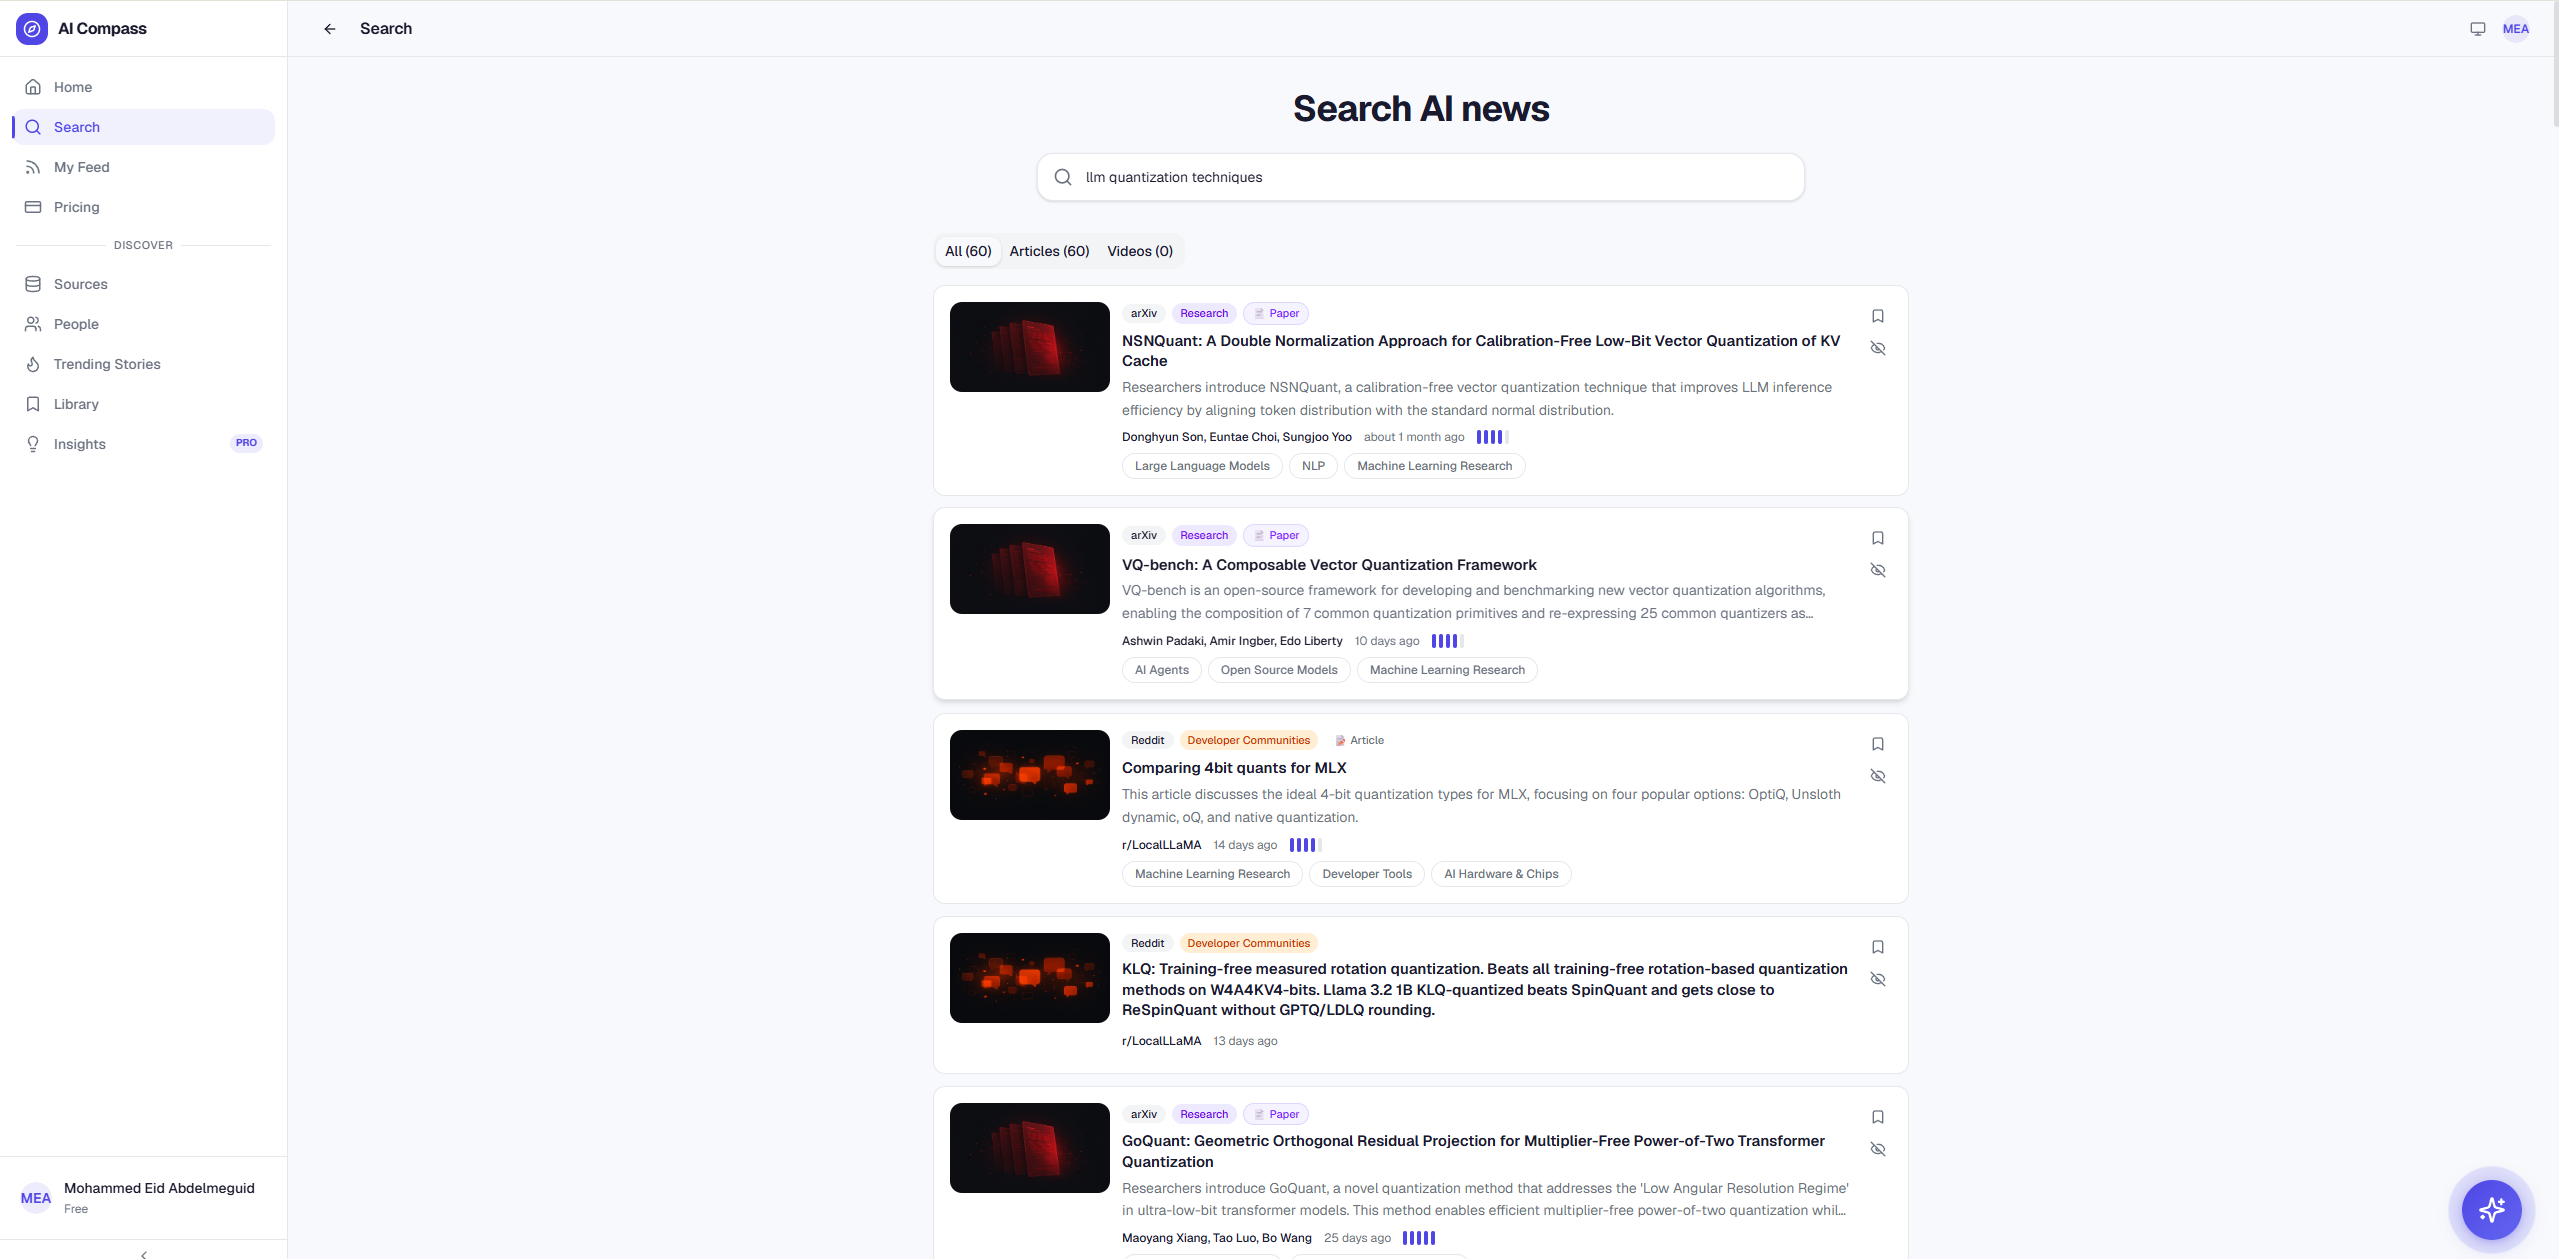
\includegraphics[width=0.85\textwidth]{figures/screenshots/screenshot_search.png}
\caption{The AI Compass search surface, showing results for the query ``llm quantization techniques.''}
\label{fig:screenshot-search}
\end{figure}

\begin{figure}[htbp]
\centering
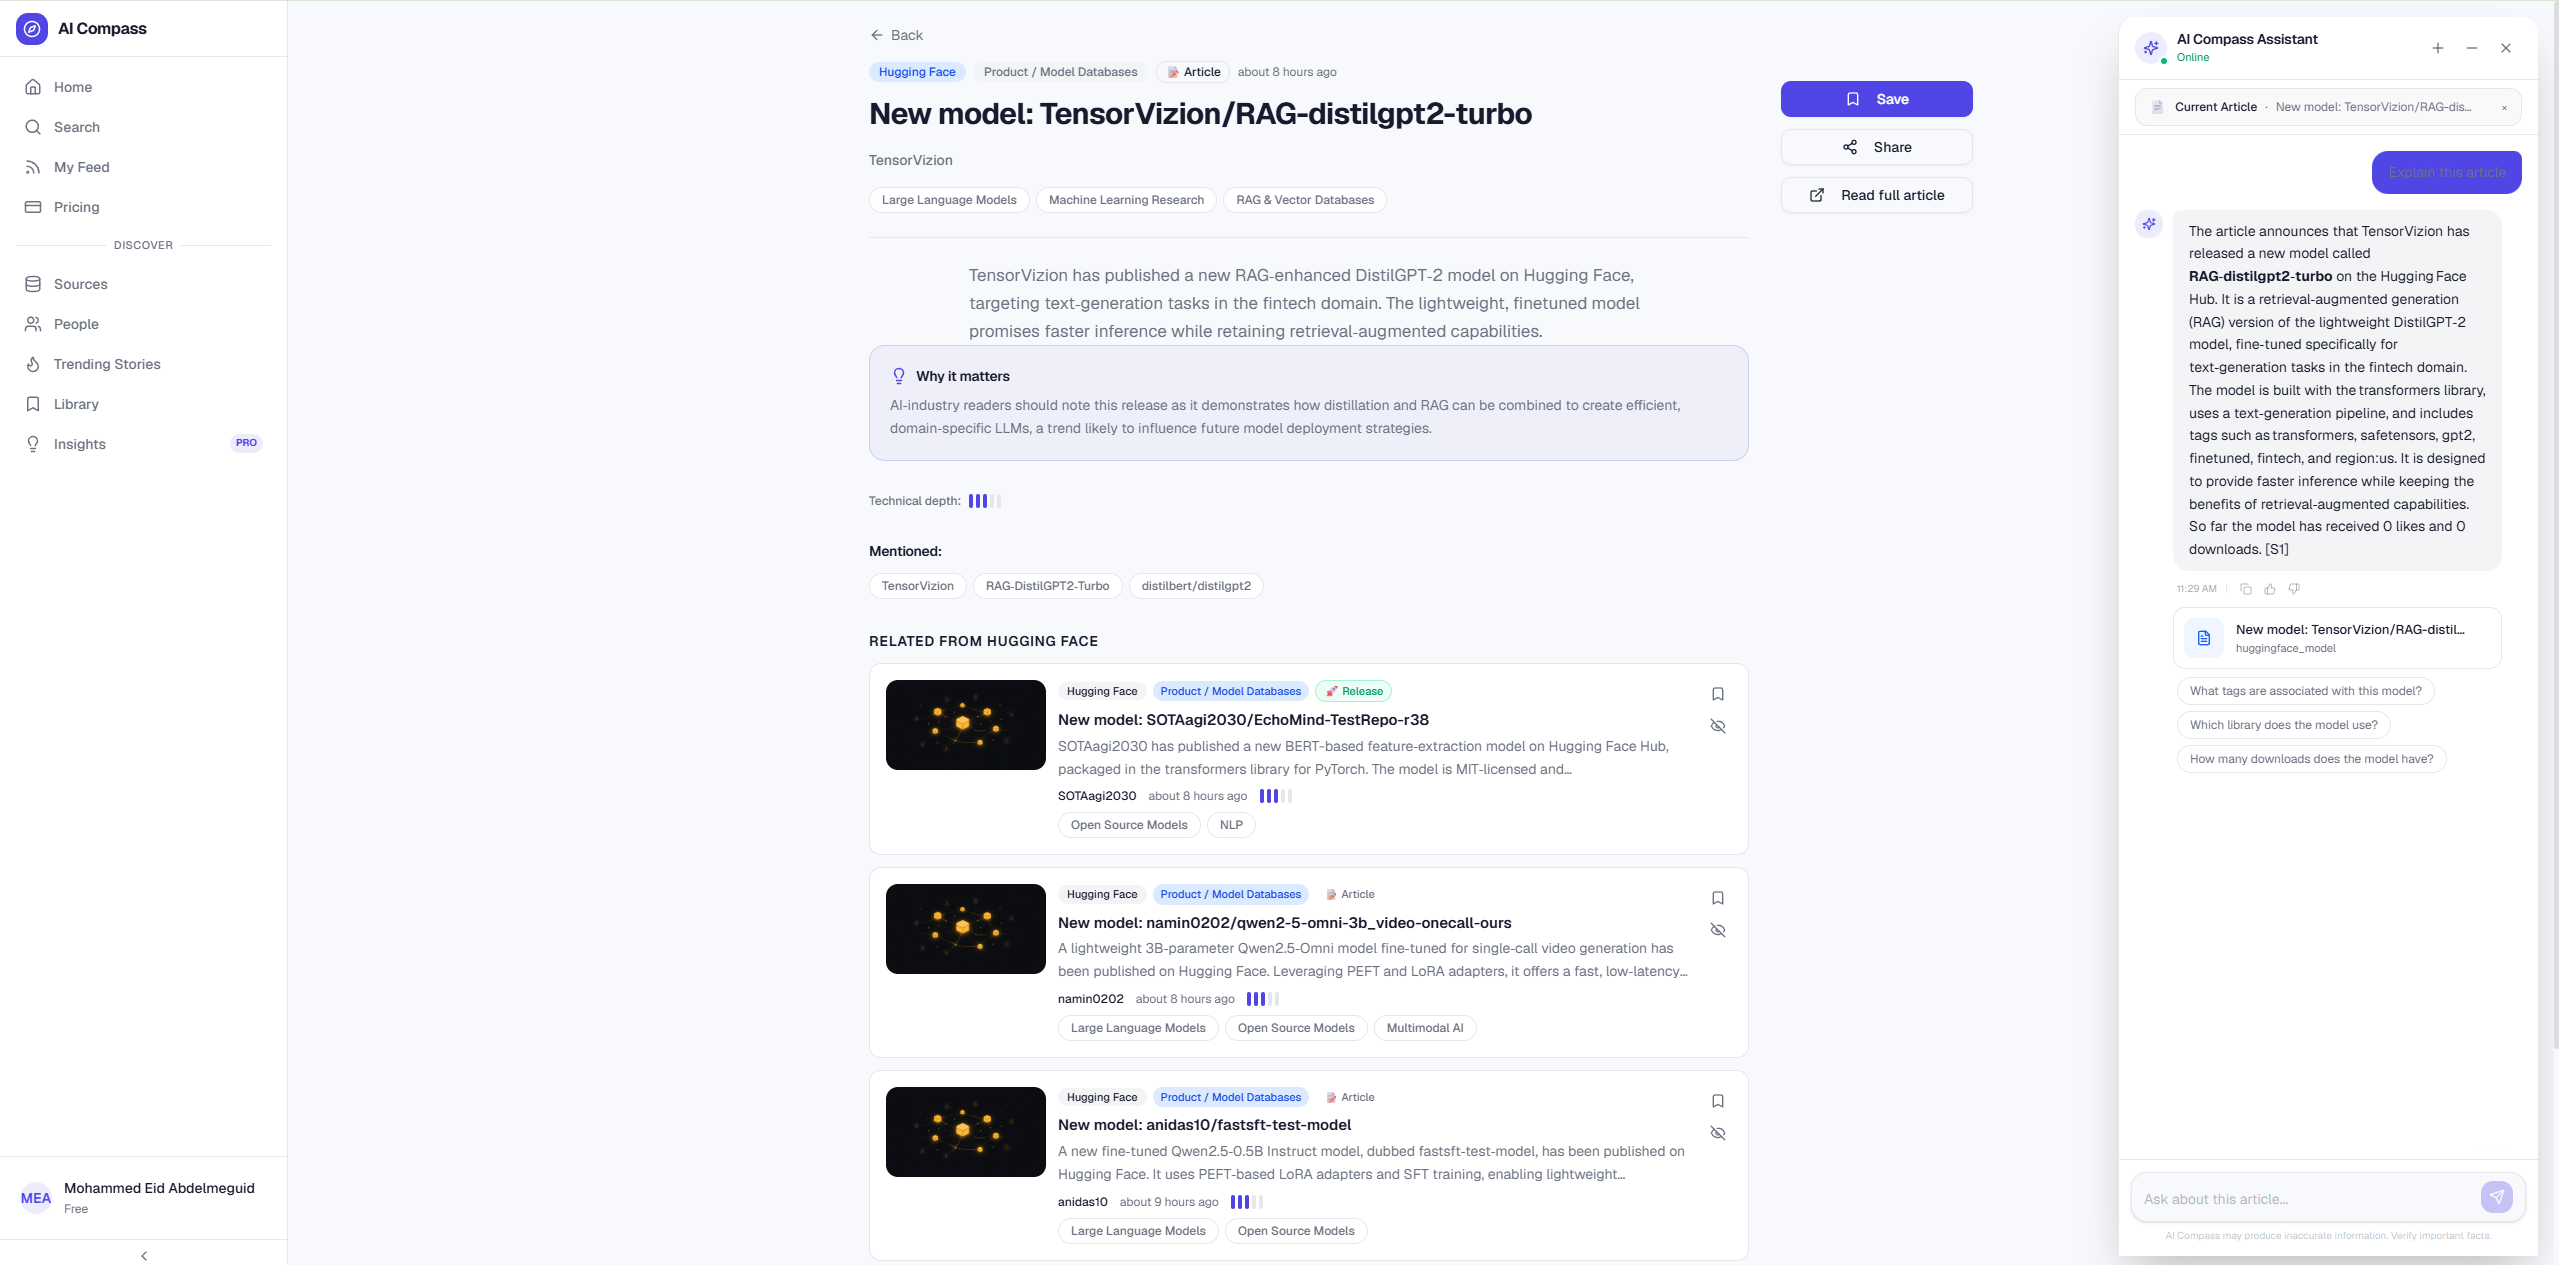
\includegraphics[width=0.85\textwidth]{figures/screenshots/screenshot_article_chat.png}
\caption{The RAG conversational assistant open alongside an article, with a numbered \texttt{[S\#]} citation resolved to a source card and follow-up suggestion chips generated by the same call (Section~\ref{sec:rag-multiturn}).}
\label{fig:screenshot-rag-chat}
\end{figure}

\section{Passage Chunking}
\label{sec:rag-chunking}

Retrieval-augmented generation operates over passages, not whole documents: a long document must be cut into smaller units before it can be embedded and searched at passage granularity, since embedding an entire document into one vector discards exactly the fine-grained detail a specific question is likely to ask about. AI Compass implements two chunkers feeding the same downstream embedding step. A sentence-based chunker is used for prose (articles): it accumulates whole sentences into a passage and carries the passage's starting and ending character offsets, later letting a citation link back to a specific span of the original text. A segment-based chunker is used for video transcripts: it accumulates transcript segments, each already carrying a start/end timestamp from the captioning or speech-to-text stage (Chapter~\ref{chap:deep-media}), and propagates those timestamps onto the resulting passage so a citation into a video can deep-link to the exact playback position (a \texttt{?t=} parameter) rather than only naming the video.

Both chunkers share the same size budget: a target passage length of $\approx$180 tokens, an overlap of $\approx$40 tokens between consecutive passages so a fact spanning a boundary is not orphaned in exactly one chunk, and a hard cap of 240 tokens. This budget exists for a concrete reason: the embedding model used throughout AI Compass, \texttt{all-MiniLM-L6-v2} (Chapter~\ref{ch:background}), silently truncates any input beyond 256 word-piece tokens rather than raising an error, so a passage embedded past that ceiling would have its tail silently discarded with no signal anything was lost. Targeting $\approx$180 with a 240 hard cap leaves a working margin under the model's true 256-token ceiling.

The project uses no real subword tokenizer (no \texttt{tiktoken} dependency); token counts are instead estimated from word counts via $\hat{n}_{\text{tok}} \approx n_{\text{words}} / 0.75$ (Equation~\ref{eq:token-heuristic}), reflecting the rough English-language rate of $\approx$1.33 word-piece tokens per word, an honest approximation, not an exact count, and stated as such here. The design does not rely on the heuristic alone for correctness: the embedding model's own 256-token truncation is the real backstop, so an under- or over-estimate produces at worst a passage a little shorter or longer than the $\approx$180-token target, never one that silently loses content, since the 240-token hard cap already sits below the model's actual ceiling.

\begin{equation}
  \hat{n}_{\text{tok}} \approx \frac{n_{\text{words}}}{0.75}
  \label{eq:token-heuristic}
\end{equation}

\section{Passage Indexing}
\label{sec:rag-indexing}

Once chunked, every passage is embedded with the same \texttt{all-MiniLM-L6-v2} model already used elsewhere in the platform (384-dimensional, run locally rather than through a hosted embedding API), and the resulting vectors are stored in a table dedicated to this purpose, \texttt{rag\_chunks}, rather than in the general-purpose \texttt{embeddings} table that the ranking and clustering subsystems already use for one-embedding-per-item vectors.

This separation is a deliberate architectural decision, not an oversight. The existing \texttt{embeddings} table is read by two other subsystems (near-duplicate clustering, Chapter~\ref{ch:data-pipeline}; ranking candidate generation, Chapter~\ref{ch:recommendation}) under an implicit but load-bearing assumption: exactly one embedding per content item. A passage-level chunk breaks that assumption outright: a single long article can produce a dozen or more chunk embeddings. Writing chunk vectors into the shared table would have silently pulled passage rows into clustering and profile-vector searches as if they were independent items, a subtle bug that would surface only as slow quality degradation, not an error. A dedicated table sidesteps this entirely: neither existing caller needs to change, or even be aware, that passage-level chunking exists.

The \texttt{rag\_chunks} table carries a pgvector index built on the Hierarchical Navigable Small World (HNSW) graph structure, using cosine distance as its similarity metric,
\begin{equation}
  d_{\cos}(\mathbf{q}, \mathbf{c}) = 1 - \frac{\mathbf{q} \cdot \mathbf{c}}{\lVert \mathbf{q} \rVert \, \lVert \mathbf{c} \rVert},
  \label{eq:cosine-distance}
\end{equation}
computed between a query embedding $\mathbf{q}$ and a candidate chunk embedding $\mathbf{c}$, with nearer neighbors (those with the smallest $d_{\cos}$) approximated by traversing the HNSW graph rather than by an exhaustive scan of every stored vector. This is the first approximate-nearest-neighbor index anywhere in the project: the pre-existing \texttt{embeddings} table, by contrast, has no ANN index of any kind, so a nearest-neighbor query against it falls back to an exact, exhaustive comparison, a limitation unrelated to the RAG assistant itself, but worth noting here because it means the retrieval path described in the rest of this chapter is, at the time of writing, the only part of AI Compass whose vector search is backed by genuinely sub-linear approximate search rather than a full scan.

\section{Retrieval}
\label{sec:rag-retrieval}

A question is first routed to one of three retrieval scopes: \emph{document} scope, when asked from a specific article or video detail page (the canonical case being ``what does this mean?'', which carries no subject of its own and must be interpreted against the page currently viewed); \emph{topic} scope, anchored to a topic rather than a single item; or an unscoped general knowledge-base query. The chosen scope can augment the query text before embedding (e.g. folding in the current page's title), and can change mid-conversation, since scope is recorded per message rather than locked to the conversation.

Once the (possibly scope-augmented) query is embedded, retrieval deliberately over-fetches $k' = \text{top\_k} \times 6$ (Equation~\ref{eq:overfetch}) candidates from the HNSW cosine search, where $\text{top\_k}$ defaults to 8, giving $k'=48$ candidates pulled back before any filtering. Over-fetching exists because the next stage (an access-control filter, Section~\ref{sec:rag-access-control}) removes an a priori unknown fraction of the result, and fetching only the final target count would risk too few, or zero, surviving passages whenever a meaningful share of the nearest neighbors belong to sources the requester cannot see.

\begin{equation}
  k' = \text{top\_k} \times 6
  \label{eq:overfetch}
\end{equation}

Surviving candidates then pass into a greedy selection step bounded by two constraints at once: a 2200-token total context budget, and a per-document diversity cap of at most 3 chunks, so one long, highly relevant document with many overlapping high-similarity chunks cannot crowd out every other relevant source.

Finally, if the filtering and selection steps leave nothing to answer with, the system does not simply return an empty context. Section~\ref{sec:rag-fallback} below describes the deterministic, non-vector fallback that recovers from exactly this case using the page the user is currently viewing, when one exists. Algorithm~\ref{alg:rag-retrieval} summarizes the full retrieval pipeline described in this section, from query embedding through to that fallback.

\begin{algorithm}[htbp]
  \small
  \DontPrintSemicolon
  \KwInput{query $q$, scope $s$, requesting user $u$, current-page document $d_{\text{page}}$ (may be null), $\text{top\_k}$ (default 8), token budget $B$ (2200), per-document cap $c$ (3)}
  \KwOutput{an ordered list of source passages $\mathcal{S}$, each carrying a citation number}
  $q' \leftarrow \textsc{AugmentByScope}(q, s)$\;
  $\mathbf{v} \leftarrow \textsc{Embed}(q')$ \tcp*{same model used to index \texttt{rag\_chunks}}
  $C \leftarrow \textsc{HNSWCosineSearch}(\mathbf{v}, k = \text{top\_k} \times 6)$ \tcp*{over-fetch, up to 48 candidates}
  $C \leftarrow \{\, c \in C : \textsc{PassesAccessControl}(c, u) \,\}$ \tcp*{Section~\ref{sec:rag-access-control}}
  sort $C$ by descending similarity to $\mathbf{v}$\;
  $\mathcal{S} \leftarrow \emptyset$; $\text{tokens\_used} \leftarrow 0$; $\text{count}[\cdot] \leftarrow 0$\;
  \ForEach{$c \in C$}{
    \If{$\text{tokens\_used} + |c| \le B$ \textbf{and} $\text{count}[\text{doc}(c)] < c_{\text{cap}}$}{
      $\mathcal{S} \leftarrow \mathcal{S} \cup \{c\}$\;
      $\text{tokens\_used} \leftarrow \text{tokens\_used} + |c|$\;
      $\text{count}[\text{doc}(c)] \leftarrow \text{count}[\text{doc}(c)] + 1$\;
    }
  }
  \If{$\mathcal{S} = \emptyset$ \textbf{and} $d_{\text{page}} \ne \text{null}$ \textbf{and} \textsc{PassesAccessControl}($d_{\text{page}}$, $u$)}{
    $\mathcal{S} \leftarrow \{\, \textsc{RawContent}(d_{\text{page}})[\,:9000\,] \,\}$ \tcp*{deterministic fallback, Section~\ref{sec:rag-fallback}}
  }
  \Return{\textsc{Numbered}($\mathcal{S}$)}
  \caption{RAG passage retrieval}
  \label{alg:rag-retrieval}
\end{algorithm}

\section{Access Control and Private Sources}
\label{sec:rag-access-control}

AI Compass lets users exclude entire sources or categories from their own feed, and subscribe to sources with restricted visibility, including ones they submitted themselves. Because retrieval draws candidates from the same shared \texttt{rag\_chunks} index for every user, nothing about the HNSW similarity search itself prevents a query from surfacing a passage the requester should never see; the access-control filter closes that gap and is a genuine, disclosed leak-prevention mechanism, not an incidental feature.

The filter applies two independent conditions to every candidate chunk. First, a chunk is dropped if its source is among the requesting user's excluded sources or categories: the same exclusion mechanism governing the personalized feed is honored here. Second, a chunk is dropped if its source is marked \texttt{visibility='user'} (submitted for private use, not curated public content) and the requester is not a subscriber, the more security-relevant condition, since without it one user's private source material could be retrieved and quoted to an unrelated user simply for being the closest semantic match.

Critically, this same filter also applies to the current-page document consulted by the deterministic fallback below: a private, unsubscribed document cannot become answerable material merely because a user is viewing its detail page.

\section{Answer Generation and Anti-Hallucination Mechanisms}
\label{sec:rag-generation}

Once a set of numbered source passages has been assembled, generation is performed by Groq's hosted \texttt{llama-3.3-70b-versatile} model, with \texttt{max\_tokens} bounded at 700 and temperature set to 0.3. The 700-token bound is the first hard \texttt{max\_tokens} limit anywhere in this codebase, a deliberate cost- and latency-control decision: an unbounded call on the project's largest model tier would expose per-message cost and latency to whatever length the model chose, rather than to an operator-capped length. The moderate, non-zero temperature (versus temperature-0 for the smaller condensation model, Section~\ref{sec:rag-multiturn}) reflects that answer generation is a synthesis task where some lexical variety is desirable, unlike condensation, which should be as deterministic as possible.

Three anti-hallucination mechanisms work together. First, the system prompt requires every substantive claim to carry a numbered \texttt{[S\#]} marker matching a supplied source, and instructs the model never to invent one, necessarily advisory, since nothing prevents a model from disregarding an instruction. Second, and server-side: every \texttt{[S\#]} marker in the returned answer is checked by regular expression against the genuinely supplied source numbers, and any marker that fails to resolve is surgically removed inline, rather than triggering a whole-sentence or whole-answer rejection; natural-language prose does not decompose into independently droppable units the way a bulleted list does, so discarding an entire sentence or answer around one bad marker would throw away legitimate cited content along with it. Third, a \texttt{grounded} boolean is set to \texttt{false} only when \emph{every} marker in the raw answer failed to resolve (the model appears to have ignored the sources entirely), remaining \texttt{true} if at least one marker resolved even when others did not, a threshold chosen so one slipped citation number does not flag an otherwise well-supported answer as ungrounded, while the all-fail case remains a strong, actionable signal.

\section{Multi-Turn Conversation}
\label{sec:rag-multiturn}

A conversational assistant must resolve a follow-up such as ``can you simplify that?'' into something retrieval can act on, since neither the phrase nor its embedding carries any information about what ``that'' refers to. AI Compass addresses this with a query-condensation step running before retrieval on every turn after the first: given the last 6 messages of history, a separate, cheaper (8B-class) Groq model at temperature 0 rewrites the follow-up into a standalone question. The rewritten question, not the literal follow-up text, is what gets embedded and retrieved against.

Because this call sits on the critical path of every follow-up turn, its failure mode is conservative: any failure falls back to the raw original question rather than blocking the turn, so a follow-up degrades gracefully to ``retrieval against the literal text'' instead of failing outright. Stored conversation history is capped server-side at 8 messages ($\approx$4 turn pairs), bounding both the condensation prompt and retained state.

A closely related feature costs nothing extra: the same generation call (Section~\ref{sec:rag-generation}) is instructed to append a trailer line \texttt{SUGGESTIONS: q1 | q2 | q3}, parsed out server-side by regex and never shown raw. Since suggestions come from the same call that produces the answer, this costs zero additional model round-trips, a feature that otherwise could have doubled per-message cost as a second, dedicated call.

\section{Streaming Architecture}
\label{sec:rag-streaming}

AI Compass exposes the assistant over two HTTP mechanisms: a conventional, non-streaming JSON endpoint returning a complete answer in one response, and a server-sent-events (SSE) endpoint streaming the answer token by token. These two paths are not deployed identically. The bulk of the Django backend (including the non-streaming chat endpoint and every other view) runs under gunicorn as a standard synchronous WSGI service with a small, fixed worker pool. Only the streaming SSE endpoint runs on a second, dedicated ASGI process (uvicorn), in its own container. It would be equally imprecise to call the backend uniformly WSGI or uniformly ASGI; the accurate statement is that the bulk of it is WSGI, and only the streaming chat path is carved out onto an isolated ASGI process.

The reason follows directly from what a long-lived streaming connection does to a small, fixed worker pool: a synchronous WSGI worker is occupied for a request's entire duration, so serving a token-by-token stream from a main-service gunicorn worker would tie it up, unavailable to any other request, for as long as the connection stayed open. Isolating the streaming endpoint means a slow or long-lived chat stream can never starve the main service's worker pool.

This split is also the one deliberate, disclosed exception to a broader principle holding everywhere else in the project: the Django web tier makes no direct LLM calls of its own, and every other LLM call happens inside the pipeline's Celery worker processes, not inside a Django request. The streaming endpoint is the exception because it needs its own lightweight Groq client living directly in Django: a Celery task boundary suits a bounded unit of work that reports back once finished, but has no mechanism for streaming individual tokens back to an already-open HTTP connection, which is exactly what SSE requires.

\section{Pipeline Summary}
\label{sec:rag-summary}

\begin{figure}[htbp]
  \centering
  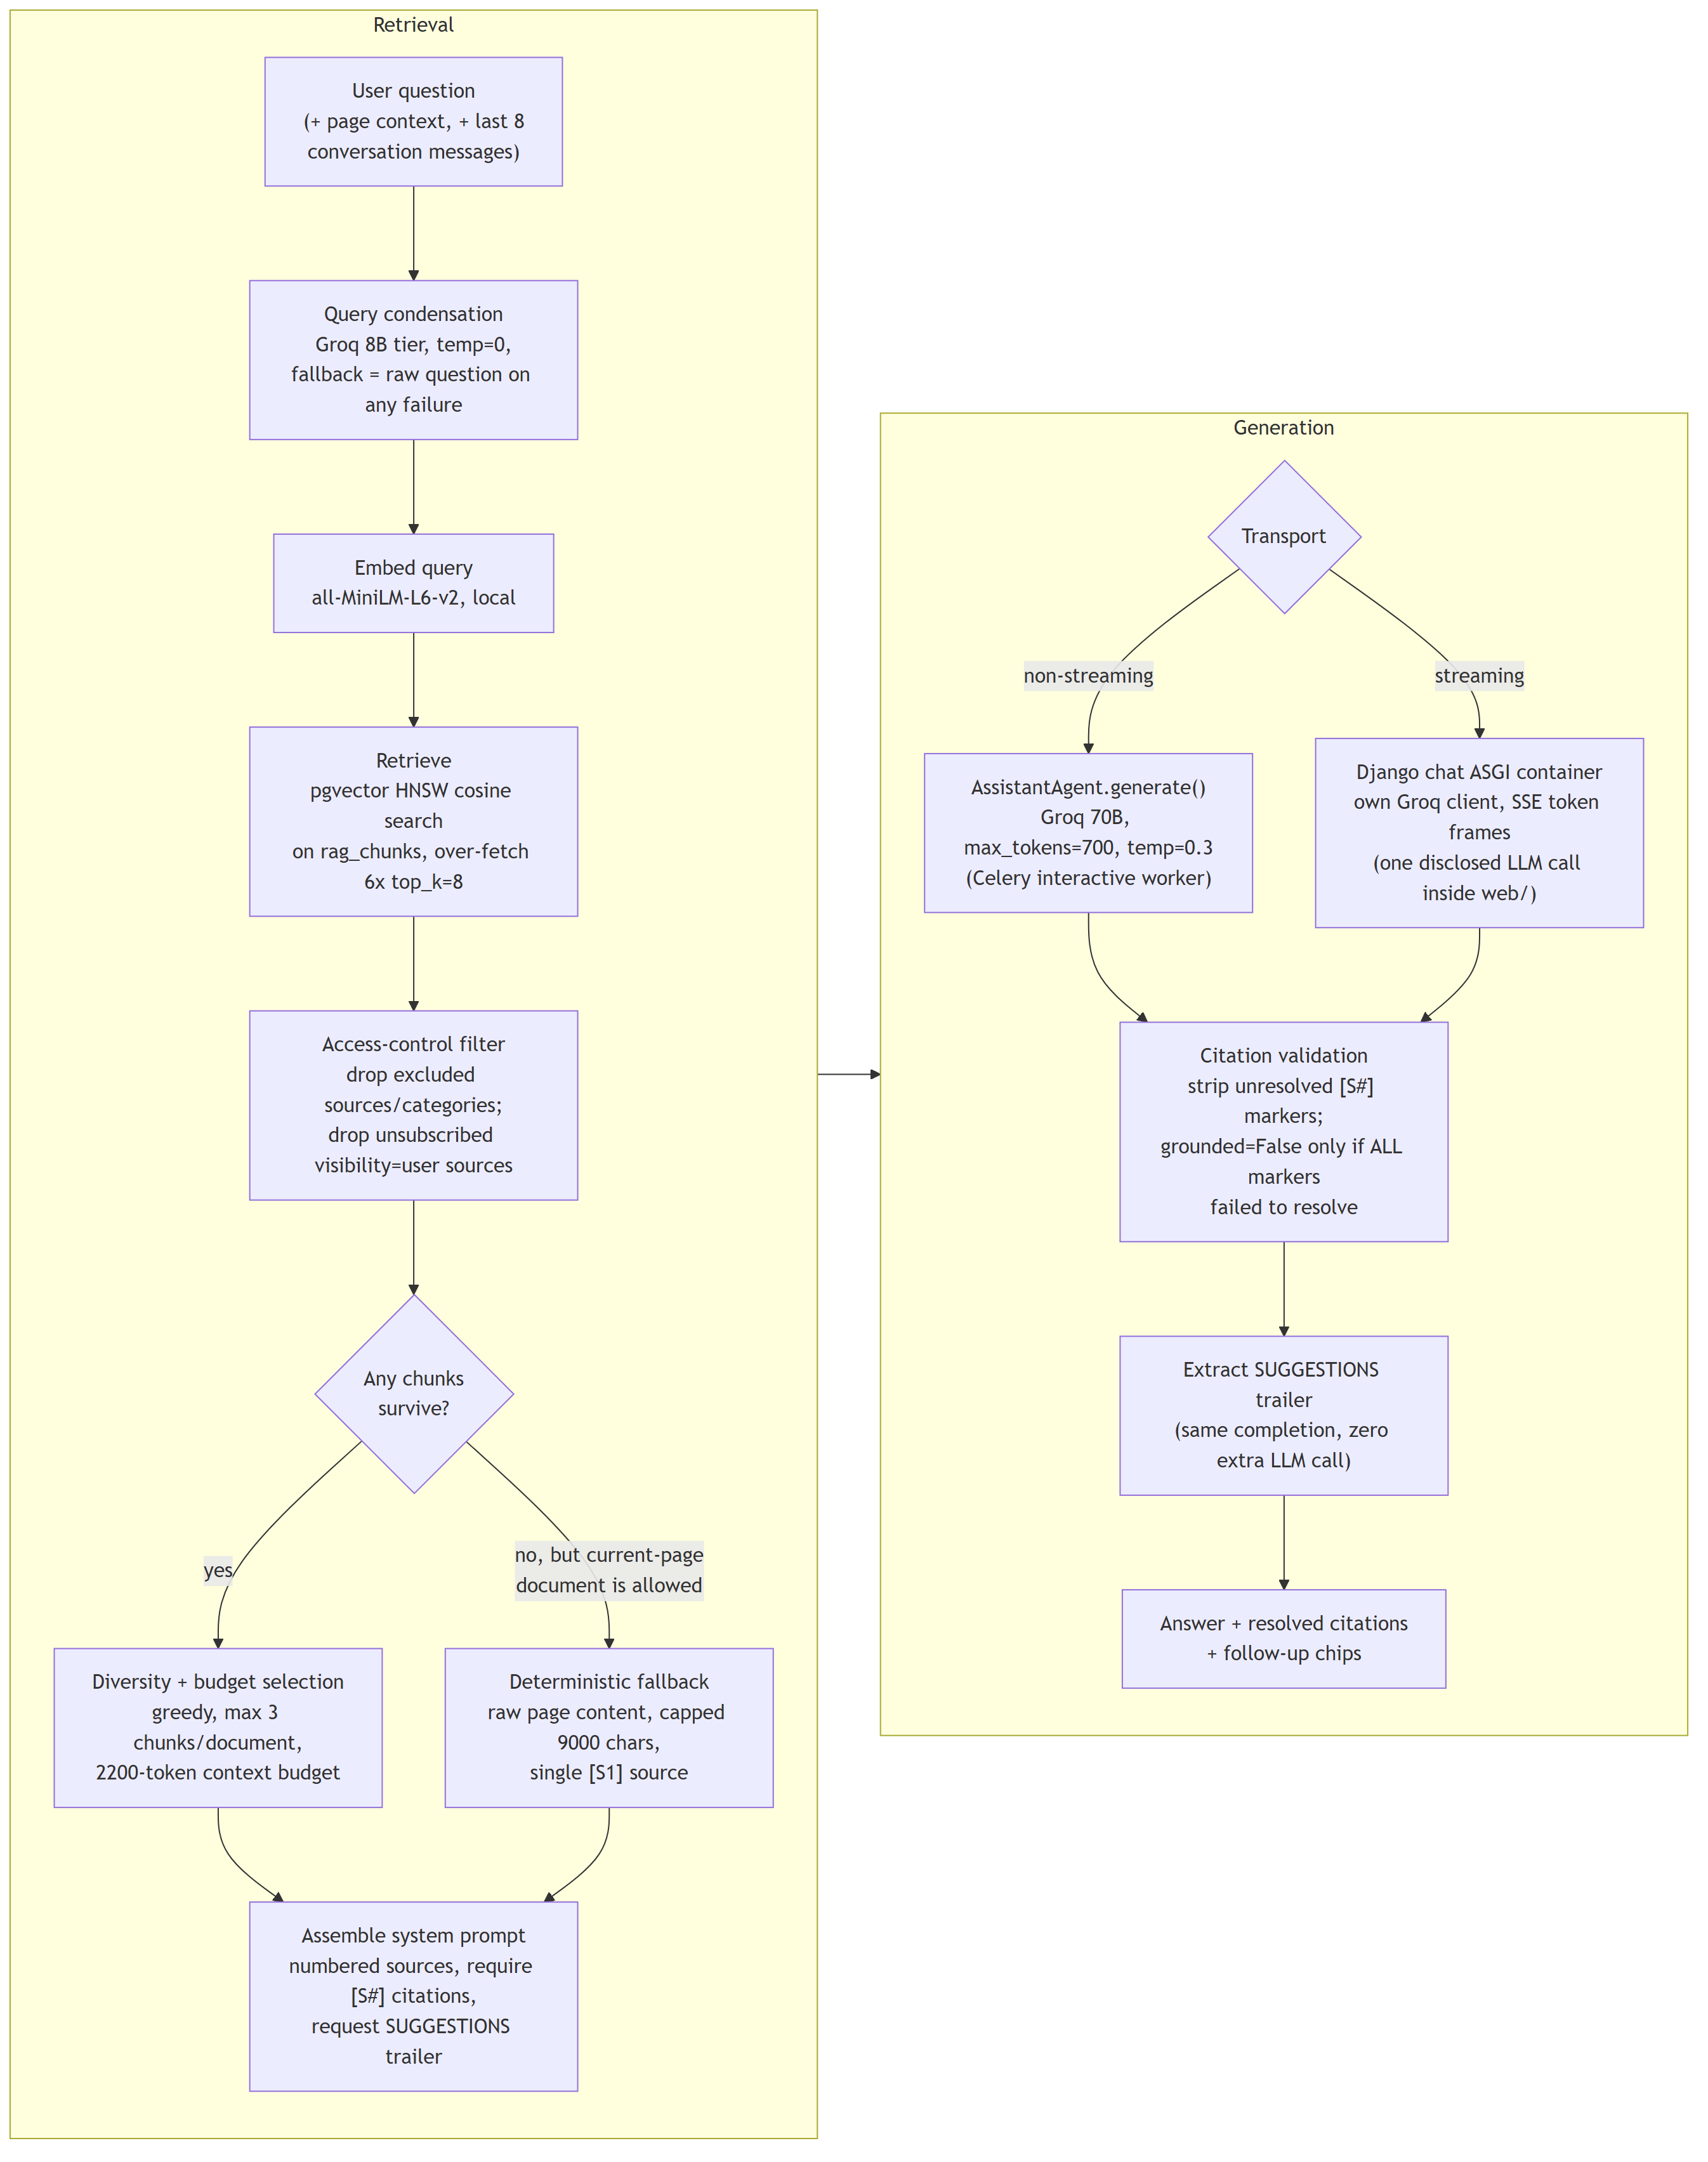
\includegraphics[width=0.85\textwidth,height=0.85\textheight,keepaspectratio]{figures/rag_pipeline.png}
  \caption{The RAG assistant's retrieval and generation pipeline, from query condensation through access-controlled retrieval to citation-validated generation.}
  \label{fig:rag-pipeline}
\end{figure}

Figure~\ref{fig:rag-pipeline} traces the full path a message takes through the assistant, drawing together every mechanism described in this chapter. A follow-up message is first condensed, with a raw-question fallback, into a standalone query (Section~\ref{sec:rag-multiturn}). The query is routed to a retrieval scope and embedded with the same model used to index passages (Section~\ref{sec:rag-retrieval}), then matched against the \texttt{rag\_chunks} HNSW cosine index with a $6\times$ over-fetch. The access-control filter removes any passage the requesting user is not entitled to see, whether by exclusion or by unsubscribed private-source visibility (Section~\ref{sec:rag-access-control}), before a greedy, budget- and diversity-capped selection assembles the final numbered source list, falling back to the current page's raw content when nothing else survives (Section~\ref{sec:rag-fallback}, folded into Algorithm~\ref{alg:rag-retrieval}). Generation then produces a citation-bearing answer and an appended suggestions trailer in a single model call, after which server-side regex validation strips unresolvable citation markers and sets the \texttt{grounded} flag (Section~\ref{sec:rag-generation}). Finally, the answer is either returned as one JSON payload or streamed token by token from the isolated ASGI process described in Section~\ref{sec:rag-streaming}, depending on which endpoint the frontend called.

\subsection{Deterministic Fallback for Freshly Indexed Content}
\label{sec:rag-fallback}

One consequence of the pipeline above is worth stating on its own, since it explains a behavior a user is likely to notice directly. If the greedy selection step in Algorithm~\ref{alg:rag-retrieval} produces an empty passage set (most commonly because a page was indexed too recently for its chunks to have propagated, or because no chunk scored highly enough to survive filtering), the system checks whether the current page's own document passes the same access-control filter described in Section~\ref{sec:rag-access-control}. If it does, that document's raw content, truncated to the first 9000 characters, is used directly as the sole numbered source for the answer, bypassing vector search entirely. This deterministic, non-vector fallback is why a question such as ``summarize this article,'' asked from an article's own detail page, reliably works even on a page freshly indexed with no other passages yet found similar to the question; the fallback does not depend on the passage index having caught up at all.

\section{Limitations}
\label{sec:rag-limitations}

Two limitations of the RAG subsystem are worth stating plainly rather than glossed over. First, no automated test coverage was found for the RAG service or its retrieval logic; this was confirmed by a repository-wide search for test files, which turned up none exercising the chunking, retrieval, access-control, or generation code paths described in this chapter. Every behavior described here has been verified by direct code reading and by manual, live, browser-driven verification sessions rather than by an automated test suite, and the absence of that suite should be read as a genuine gap rather than an implicit claim of tested correctness.

Second, the deterministic fallback described in Section~\ref{sec:rag-fallback} is itself only a partial remedy for a freshly indexed or otherwise poorly matched document. Its 9000-character cap means that a document substantially longer than that is only partially visible to the assistant even while the fallback is active: the model is given the first 9000 characters of the page's raw content, not the whole document, so a question whose answer depends on material past that cutoff can go unanswered by the fallback in exactly the same way it could by an incomplete vector-search result. The fallback closes the specific gap of ``nothing was retrieved at all''; it does not, by itself, guarantee that the entirety of a long document is available to the model.
